\documentclass[10pt,draftclsnofoot,onecolumn]{IEEEtran}

\usepackage{setspace}
\usepackage{caption}
\usepackage{hyperref}

\hypersetup{
    colorlinks,
    citecolor=black,
    filecolor=black,
    linkcolor=black,
    urlcolor=black
}

% *** GRAPHICS RELATED PACKAGES ***
\ifCLASSINFOpdf
  \usepackage[pdftex]{graphicx}
  % declare the path(s) where your graphic files are
  \graphicspath{images/}
  % and their extensions so you won't have to specify these with
  % every instance of \includegraphics
  \DeclareGraphicsExtensions{.pdf,.jpeg,.png}
\else
\fi

% correct bad hyphenation here
\hyphenation{op-tical net-works semi-conduc-tor}

\begin{document}
\pagenumbering{gobble}
\singlespacing
\title{Spatial Visualization\\ of Biodiversity}

\author{Ty~Skelton,
        Jasper~LaFortune,
        and~Alex~Shields}% <-this % stops a space

% The paper headers
\markboth{CS 461}%
{Spring 2016}

% make the title area
\maketitle

% As a general rule, do not put math, special symbols or citations
% in the abstract or keywords.
\begin{abstract} %
The Department of Integrative Biology at Oregon State has collected a large sample of biodiversity data from various sites in the Southwest United States.
Handling this data in its raw form requires certain technical knowledge of databases, as well as a bit of patience.
This presents a problem for biodiversity researchers and Department of Defense land managers, who need to be able to understand and make decisions about this data easily.
Our team addressed this problem by creating a web interface for spatially visualizing this data.
We enabled users to easily display useful graphs and maps about areas and species of interest, putting the information they care about most at their fingertips.

The Department of Defense made an investment in collecting all these samples so that it could better manage its land.
However, extracting meaning from that information is challenging for land managers and researchers alike.
Any good solution to this problem would allow users to easily access the information that is important to them.
Our solution provides an interface that allows users to select information of interest and see it in map and graph form.
Passerby at Expo will be invited to interact with our system and discover meaningful biodiversity patterns for themselves.
Oregon State biodiversity researchers have indicated that our product meets their needs.

\end{abstract}
\IEEEpeerreviewmaketitle

\newpage
\tableofcontents
\newpage
\pagenumbering{arabic}
\section{Introduction} % @TODO: Jasper
% Who requested it?
% Why was it requested?
% What is its importance?
% Who was/were your client(s)?
% Who are the members of your team?
% What were their roles?
% What was the role of the client(s)? (I.e., did they supervise only, or did they participate in doing development)
% Who requested it?
% Why was it requested?
% What is its importance?
% Who was/were your client(s)?
% Who are the members of your team?
% What were their roles?
% What was the role of the client(s)? (I.e., did they supervise only, or did they participate in doing development)
Professor Dave Lytle, head of the Lytle Lab in the Department of Integrative Biology at Oregon State University, requested this project.
His research team had collected five years of insect samples from Department of Defense bases and amalgamated the observations into a large, somewhat messy database.
He asked our team for a visualization system to help make sense of the data.
Such a system would aid researchers in data analysis, and help the Department of Defense to make informed land management decisions.
Dr. Lytle and his research team sponsored the project and acted as clients for the product.
We met with them periodically throughout each term to go over progress and goals.
They were, of course, involved in design decisions, but left the implementation details primarily to us.

Our team consists of Jasper LaFortune, Alec Shields, and Ty Skelton.
We each had a distinct role in development and team leadership.
Jasper 	developed the Filter View 	and led the team's presentations, 			including organizing the poster, video reports, and elevator pitch.
Alec 	developed the Map View 		and led the team's external communications, including contacting our clients and submitting assignments.
Ty 		developed the Graph View 	and led the team's internal communications, including organizing meetings and individual tasks.
Development and leadership responsibilities were shared fairly among all three members.


\newpage
\section{Original Requirements} % @TODO: Ty
% This needs to be the original document, showing what you thought, at the time, was the project definition.
% This needs to include the original Gantt chart.
\subsection{Project Description}

\par This project will deliver a web application that will be used to interactively visualize biodiversity data.
This application will be used by researchers and Department of Defense land managers to compare and analyze biodiversity data in areas of interest.

\subsection{Service Need}

\par Professionals working out in the field on government-owned property are tasked with preserving the ecosystems within them.
To serve this purpose, they’ve requested a tool with which they can quickly assess biodiversity levels of different key areas.

\subsection{Client Requirements}

\par Our client will provide us with the data to visualize and a web server on which to host the application.
\begin{list}{-}{}
\item The dataset will provide each individual observation of an insect, including the location, time, and taxa of the species observed.
\begin{list}{-}{}
\item The location will be one of about 700 sites in the Southwestern United States, and will include latitude and longitude.
Sites are hierarchically organized in that each site belongs to a basin.
\item The time will be between 2009 and 2013.
Samples were collected at individual sites anywhere from only once to twice a year.
\item The taxa will be the fully qualified taxonomy of the insect species observed.
These will be hierarchically organized, as every species belongs to a genus, which belongs to a family, and order, and so on.
\end{list}
\end{list}

\subsection{Functional Requirements}

\par We will create a web interface for interacting with and visualizing the dataset provided to us.
This interface will provide three views:

\begin{list}{-}{} % main list

\item Map View

\begin{list}{-}{}
\item This view will display a map, annotated with markers at the locations of all the sites where data have been collected.
\item Users will be able to pan and zoom in this view.
\item They will also be able to select a site in this view by clicking on it.
\item As a stretch goal, we will display markers with size or color according to biodiversity metrics of that site.
\end{list}

\item Statistics View

\begin{list}{-}{}
\item This view will display useful summary statistics, graphs, and charts about the selected information.
These will include:
\begin{list}{-}{}
\item A graph of biodiversity over time.
\item The Shannon diversity score.
\item A chart of insect population by taxa or species.
\end{list}
\end{list}

\item Filter view
\begin{list}{-}{}
\item This view will allow the user to filter what information is displayed in the Map and Statistics Views.
It will contain:
\begin{list}{-}{}
\item Date filter
\begin{list}{-}{}
\item This will allow the user to select data from a range of dates.
\end{list}
\item Taxa filter
\begin{list}{-}{}
\item This will allow the user to select multiple taxa (e.g. species, order).
\item The species will be organized hierarchically within the pane.
\end{list}
\item Site filter
\begin{list}{-}{}
\item This will allow users to select multiple sites.
\item The sites will be organized hierarchically (into their containing basins) within the pane.
\end{list}
\end{list}
\end{list}

\item STRETCH GOAL Advanced statistical analysis
\begin{list}{-}{}
\item As a stretch goal, this feature will go beyond the data manipulation implemented in the different graphing features of the main app.
We will work with David Lytle and his team to generate advanced statistical models on the data they’ve gathered.
Since this is a stretch goal, it is currently undefined and will only be reached once we complete the 1.0 version of our website.
\end{list}
\end{list}

\subsection{Technical Requirements}

\begin{list}{-}{}
\item Set up mapping tool
\begin{list}{-}{}
\item Set up a mapping tool (e.g. ArcGIS) to create the map view.
\end{list}
\item Test cross-browser support
\begin{list}{-}{}
\item We will test our application to support common browsers such as Chrome, Firefox, Internet Explorer, and Edge.
\end{list}
\item Set up web server
\begin{list}{-}{}
\item We will set up a web server to host our application. We will either acquire a server or use a web hosting service.
\end{list}
\item Set up website
\begin{list}{-}{}
\item We will create a base website to house our application.
We will build this with a web framework to do the heavy lifting for basic needs such as user control, security, database access, and templating.
\end{list}
\item Set up database
\begin{list}{-}{}
\item We will get this data in its raw form from our client.
We will then convert their data into a form that can be stored in a relational database.
\end{list}
\item Create In-depth documentation
\begin{list}{-}{}
\item We will provide sufficient technical documentation of our application for another developer to make extensions and additions to it.
\end{list}
\end{list}

\subsection{Communication Plan}
\par We will use the following for our internal communication:
\begin{list}{-}{}
\item Slack
\begin{list}{-}{}
\item We will use this chat client for coordinating meeting times.
\end{list}
\item GitHub
\begin{list}{-}{}
\item We will keep version control of our code on GitHub.
\end{list}
\item Regular meetings several times a week
\begin{list}{-}{}
\item In order to make regular process towards goals that have been assigned and set by ourselves, we will meet regularly and consistently re-evaluate our progress.
\end{list}
\end{list}

\par We will use the following for our external communication:
\begin{list}{-}{}
\item Email will be our primary means of contact with our client.
\item We will meet twice a month with our TA.
\item We will meet twice a month with our client.
\end{list}

\subsection{Documentation}
\par Technical Documentation will be provided by the following:
\begin{list}{-}{}
\item Microsoft Sharepoint
\begin{list}{-}{}
\item As per our class requirements, we’ve created a sharepoint site that will be the primary form of providing updates on progress and holding all revisions of our code base and documentation.
This is shared amongst the client, the developer team, and the professor/TAs.
\end{list}
\item Github
\begin{list}{-}{}
\item While the sharepoint site will be where all code versions will be hosted officially, Github will be the tool the development team will use for version control internally.
Documentation will be held here as well, but replicated in the sharepoint site.
\end{list}
\end{list}

\subsection{Timeline}
Timeline showed in Fig \ref{fig:original_gantt}.
\begin{figure}[h]
\centering
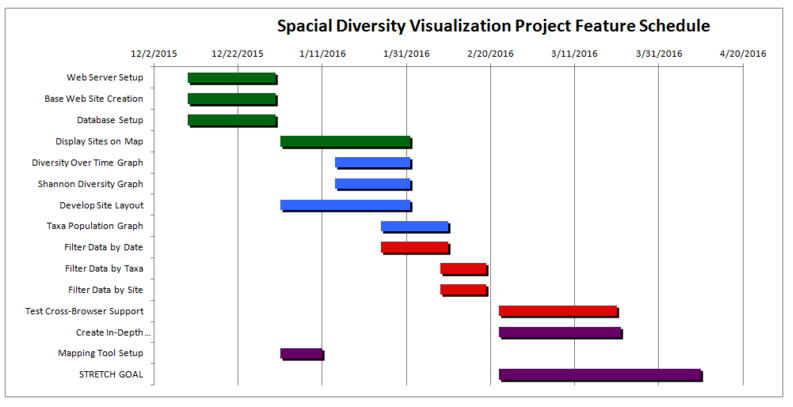
\includegraphics[width=0.9\textwidth]{OriginalGantt.png}
\captionsetup{justification=centering}
\caption{
  This is our original speculated gantt chart.
  It displays the time estimates that we had originally assumed various required tasks would take.
  As you can see it had a fairly smooth flow to it, which we learned soon in was very different in practice.
}
\label{fig:original_gantt}
\end{figure}

\subsection{Signature}
This looks good to me as a starting document. It doesn't have much about the Obj 2 statistical parts, but we can add those later. Consider this email my signature on the document.
Dave+
*************************************
David A. Lytle
Oregon State University
(541) 737-1068


\newpage
\section{Changes to Original Requirements} % @TODO: Alex
% What new requirements were added? What existing requirements were changed? What existing requirements were deleted? Why?
% Use the following table format:
% What was the final Gantt chart? @TODO: Ty
Resulting gantt chart shown in Fig \ref{fig:final_gantt}
\begin{figure}[h]
\centering
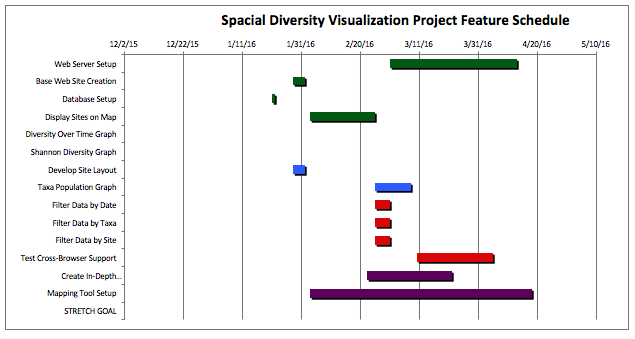
\includegraphics[width=0.95\textwidth]{FinalGantt.png}
\captionsetup{justification=centering}
\caption{
  Our resulting gantt chart after tracking the assign and completion dates for issues in Github.
  When comparing it to our speculated Gantt chart it is much less waterfall-esque, but taught us a valuable lesson in how sometimes certain aspects have to come before others.
}
\label{fig:final_gantt}
\end{figure}

\newpage
\section{Original Design Document} % @TODO: Alex
% Your original design document. Also, a discussion of what had to change over the course the year.

\newpage
\section{Tech Review} % @TODO: Jasper
% Your original design document. Also, a discussion of what had to change over the course the year.
Our original Technology Review is included below, along with notes about changes made over the course of the year.
% Your original design document. Also, a discussion of what had to change over the course the year.


%%%%%%%%%%%%%%%%%%%%%%%%%%%%%%%%%%%%%%%%%%%%%%%%%%%%%%%%%%%%%%%%%%%%%%%%%%%%%%%%%%%%
\subsection{Relational Database}

\subsubsection{MySQL}
MySQL is an open-source relational database management system (RDBMS). 
It is the most widely used open-source client-server model RDBMS. 
The source code is available under the GNU General Public License. 
The members of our team have the most experience using this database technology and it’s quite easy to use, which means the initial learning curve will be quite low. 
MySQL is also compatible with almost every operating system, which makes it quite portable in the event of an environment change. 

While the benefits to using MySQL appear to be substantial, members of the tech community have voiced various complaints. 
Among these are issues with scalability, continuation of development, and limitations. 
The scalability of MySQL seems to take a hit with increase write/read ratio. 
This isn’t enough to steer large companies and start-ups from using this technology, so we will take that with a grain of salt. 
The lagging continuation of development and limitations stems from an issue with it’s duality of being open-source and owned by Oracle. 
The code base as stagnated slightly and as a result MySQL hasn’t grown much for some time. 
This isn’t an immediate issue for our team, however, because the features it does have are exactly what we need. 
We will still compare this tool against the other potential database technologies to make sure we make the right choice. 

\subsubsection{Postgres}
Postgres is also an open-source database technology and is an object-relational database management system (ORDBMS). 
Unlike MySQL, the source code is available only under the PostgreSQL License. 
No members of our team have used this technology yet, but from skimming the documentation it does not look too foreign and could most likely be learned while developing the site. 
Postgres operations have been said to be faster than that of MySQL.

While Postgres can be faster at times and scale better than MySQL when using it concurrently, it still has its disadvantages. 
When executing many read-heavy operations, Postgres can be overkill and actually less performant than MySQL. 
Postgres has a strong community behind it, but it’s not as large as MySQL and is far less popular. 

\subsubsection{MongoDB}
MongoDB is also an open-source database, but rather than being a variation of a RDBMS database it’s a document-oriented database. 
Document-oriented databases are also known as ‘NoSQL’ databases, which casts aside the traditional relational-database structures supported by MySQL and Postgres and insteads supports JSON-esque documents (called BSON). 
MongoDB is available under the GNU Affero General Public License and the Apache License. 
If implemented correctly using the document format, MongoDB can be much faster than it’s RDBMS counterparts. 
The most advertised benefit to using a NoSQL database like MongoDB is the fact that it is very flexible, due to the fact any entity can have any attributes. 

Being flexible is a very nice feature for a database technology, especially when you’re unsure of the data types coming in. 
However, we have a fairly static data pool already and we know exactly where things will be and the structure probably will never change. 
This means that MongoDB might be fun to consider if the performance boost outweighs the benefits of the other database technologies, but it’s probably not the right tool for the job. 

\subsubsection{MariaDB}
MariaDB is a fork off of the MySQL database. 
The fork off of the major code repository was in response to the Oracle acquisition. 
MariaDB was designed for ‘drop-in’ compatibility when replacing MySQL in existing systems. 
It is almost identical to MySQL except for a few minor differences. 
The most prominent of these is the fact that it’s got a larger open-source community behind it. 
Secondly, it requires a bit more memory due to it’s default enabling of the Aria storage engine that handles internal temporary tables. 
Outside of those, the differences are very technical and minor. 

\subsubsection{Selection}
After careful consideration, we’ve chosen MySQL as our database technology for this project. 
It’s offers the same level of verbosity as the rest of the tools, while being supported in an open-source and proprietary context. 
The relational structure of MySQL caters to our data set and will be easy to manipulate and query. 
MySQL’s portability across all major operating systems is very enticing and will prove to be very helpful in the event that we have to change hosting services or move it to a remote server. 
Finally, our teams base familiarity with the tool was a convenient plus and will ideally remove whatever potential overhead for learning a database tool during our development. 


%%%%%%%%%%%%%%%%%%%%%%%%%%%%%%%%%%%%%%%%%%%%%%%%%%%%%%%%%%%%%%%%%%%%%%%%%%%%%%%%%%%%
\subsection{Backend Web Framework}

\subsubsection{Django}
Django is a free and open-source web framework written in Python. 
It’s major design philosophy is that you should be able to focus on developing your application without needing to focus on the intimate details. 
It seeks to create this environment by offering a clean and easy to use framework with various components encapsulate the different functionalities that you need to run a web application. 
It comes out of the box with various components that make it simple to start working on your application right away such as: a standalone web server for development, an interface for administration, and built-in protection from various kinds of web attacks. 
These are only part of the default modules, there are many third-party packages that can be plugged into Django that add even more powerful features such as site-wide search or content management. 
Overall, the framework seems to be about taking your mind of the web side of things so that you can focus on making your application.

\subsubsection{Symfony}
Symfony is a free PHP web application framework. 
It is focused on creating a platform that can be set up easily for a small application but is robust enough to support large and complex applications as well. 
It also seeks to give developers full control over the configuration and customization of their project. 
Another principle it operates on is DRY, Don’t Repeat Yourself, and it implements this by the way of bundles. 
Everything in Symfony is wrapped in a bundle that can be reused in other applications. 
For instance if you make everything you need to interact with a certain database you can keep that in its own bundle that you could use in two different applications that needed that database. 
Even the core of symfony is essentially a collection of bundles that you can mix, match, and modify as you see fit. 
There is also a large and active community of developers creating and collaborating on open source bundles. 
These can greatly reduce development time on a project because you often don’t have to create generic functionality from scratch.

\subsubsection{Laravel}
Laravel is a free and open source PHP web application framework. 
Similar to Symfony is it based on a modular package based system. 
In fact, Laravel has a very similar approach to Symfony, it uses many of the same tools and technologies and even uses parts of symfony itself. 
 Laravel differentiates itself from Symfony in two major ways: being very simple and easy to setup and the focus on elegant and clear syntax. 
 Even the Symfony website talks about how Laravel takes the pain out of common tasks associated with web development. 
Laravel is in my mind the PHP equivalent of Django in that it seeks to create an elegant and simple way to create web application without having to deal with the dirty details.

\subsubsection{Selection}
We have decided to use Django for our project. 
Even though our group members have experience using the other two frameworks, we have gone with Django for several compelling reasons. 
The operating system was a significant factor. 
Python is a very clean and elegant language that had thought and foresight put into its design. 
PHP, on the other hand, has somewhat of a reputation as a language that it very ugly, messy, and unguided. 
 Cleanliness is not the other reason for preferring Python, though. 
 Many of our mathematical and statistical modules will be in Python so it will be preferable to work in the same language as much as we can. 
 Another factor is the ease of starting a project with Django. 
 It is simply a handful of commands and you have your fresh project ready with a development webserver all set up. 
 With Symfony setup can be a long arduous process as you set up all the individual pieces and try to understand how to get them all to work together properly. 
 Symfony definitely offers more customization and power, but our application is small project that won’t need to take advantage of that power. 
 In the end it was closest between Django and Laravel but Django wins due to being Python instead of PHP.


%%%%%%%%%%%%%%%%%%%%%%%%%%%%%%%%%%%%%%%%%%%%%%%%%%%%%%%%%%%%%%%%%%%%%%%%%%%%%%%%%%%%
\subsection{Numerical Analysis}

\subsubsection{MATLAB}
MATLAB deserves to be mentioned here, as it is the most commonly used scientific computing language. 
It provides a tremendous amount of functionality for scientific computing needs. 
If the numerical analysis portion of our project were completely standalone, MATLAB would be an excellent choice. 
However, we can’t run it on a backend server, especially one that talks to our web framework.

\subsubsection{Numpy/Scipy}
Numerical Python, or NumPy, combined with Scientific Python, or SciPy, is the authoritative set of Python packages for scientific computing. 
NumPy is organized around the ndarray object, which is essentially a more Pythonic version of an array. 
They are distinct from Python lists in that they do not hold arbitrary objects (unless you explicitly ask them to, in which case you are probably using them wrong). 
While Python lists make no assumptions about the homogeneity of the data they are storing, NumPy ndarrays optimize based on the assumptions that each entry contains the same fields of the same types, and the entries are organized into a square n-dimensional matrix. 
These simplifications turn out to cover the vast majority of scientific applications, and allow NumPy ndarray objects to use C structures under the hood. 
This makes them efficient in memory usage and fast in processing compared to plain Python objects. 
On top of the ndarray object, the NumPy and SciPy modules provide functions for many common mathematical, statistical, and scientific routines. 
The libraries cover everything from element-wise arithmetic to linear algebra in single function calls, such that users will rarely have to explicitly iterate through an ndarray object element by element. 
More advanced specific capabilities can be offered by modules such as OpenCV, but many of these make use of NumPy ndarrays. 
Finally, NumPy and SciPy have excellent documentation and support. 
In short, NumPy and SciPy are Python’s answer to MATLAB. 
They should be more than adequate for our project.

\subsubsection{SciRuby}
SciRuby happened because some people went, “Hey, where’s the scientific computing for Ruby?” and started a GitHub repo. 
The project is still young, but provides an impressive smattering of scientific computing tools. 
In addition to providing most of the same basic array manipulation functionality as NumPy and MATLAB, SciRuby has built in functionality for some advanced routines, including several machine learning methods. 
It even includes some visualization tools, which would be of use to us if it were on the frontend. 
However, SciRuby has scattered, inconsistent documentation and support. 
Many of the modules it offers are not currently stable. 
One cannot simply assume that a SciRuby package just works.

\subsubsection{PEAR}
PEAR, or the PHP Extension and Application Repository, is a collection of PHP snippets that developers have built and which seem useful. 
It includes everything from user authentication to some scientific computing routines. 
Each extension must be found and installed separately, and there is not necessarily any consistency between extensions. 
It is about all PHP has to offer for numerical analysis.

\subsubsection{Selection}
We have chosen to use NumPy/SciPy for the numerical analysis piece of our project. 
This option should provide us with the greatest ease of development for several reasons. 
First, NumPy and SciPy are consistent. 
They are well-documented, well-tested, and well-supported. 
In general, if think NumPy should be able to do it, it already does, and one can guess what the function is called and how to use it. 
If not, it can reliably be found in the documentation. 
The only other technology which provides this ease of development is MATLAB, which is not suitable for a backend server. 
NumPy and SciPy also enjoy the advantage of being able to talk easily with our website backend, which will use Django.


%%%%%%%%%%%%%%%%%%%%%%%%%%%%%%%%%%%%%%%%%%%%%%%%%%%%%%%%%%%%%%%%%%%%%%%%%%%%%%%%%%%%
\subsection{Mapping API}

\subsubsection{Google Maps}
The Google Maps API provides all the functionality of the Google Maps app as an API that is (pretty much) free to developers. 
This means that developers can, for example, easily and simply create a map, scale and transform it, place markers on it, and make those markers display further information. 
Common use cases such as these are simple to implement. 
Furthermore, they are simple and easy for users to understand. 
Customization, for both developers and users, is a greater challenge. 
The Google Maps API follows Google’s principles in general: for 99\% of use cases, it is simple, easy, and elegant, and for the other 1\%, it is useless.

\subsubsection{ArcGIS}
ArcGIS is a powerful mapping tool commonly used for geospatial applications and research. 
It provides a JavaScript API for developers. 
The API is well-documented and includes understandable code samples. 
Advanced tools for visualization and analysis are built in, as well as nice tools for information visualization in separate windows or panels. 
It even includes a tool for visualizing watersheds, which could be of direct use to our application, and which would be very challenging to implement ourselves. 
It does require a license, but that license is available free to Oregon State faculty and students. 

\subsubsection{CartoDB}
CartoDB is a powerful map-based visualization tool, heavily centered around its JavaScript API. 
The API is not as well-documented as that of ArcGIS, but it does include useful sample code. 
It provides tools for viewing maps and visualizing and analyzing data. 
It is designed for big datasets. 
CartoDB provides similar functionality base functionality to ArcGIS, but with less advanced functionality. 
The free plan is reasonable, but premium plans are expensive, and do not come with Oregon State tuition.

\subsubsection{Selection}
We have decided to use ArcGIS for our mapping API. 
It implements many of the features we already know we want, which sets it apart from the Google Maps API. 
Additionally, we will already have the license to use it at no financial cost, which sets it apart from the CartoDB API. 
Furthermore, ArcGIS will be familiar to researchers in the field, which is important for our project. 
Finally, the API is well-documented and easy to navigate, which will improve ease of development.


%%%%%%%%%%%%%%%%%%%%%%%%%%%%%%%%%%%%%%%%%%%%%%%%%%%%%%%%%%%%%%%%%%%%%%%%%%%%%%%%%%%%
\subsection{Graphing Utility}
\subsubsection{D3}
D3 allows you to bind arbitrary data to a Document Object Model (DOM), and then apply data-driven transformations to the document. 
D3 provides powerful data-driven visualization. 
This means that we can perform minor statistical manipulation to the data pulled from the database in real-time via a view on our website. 
This is incredibly useful, because users on the site will be able to make selections on what data they’re interested in and the analysis should change with those selections. 
D3 uses HTML, SVG, and CSS. 
This technology is able to be implemented with any web framework and only requires either a reference to a remote CDN or a local install of the source files. 
D3 can also work with any data size, even performing while in the Gigabits range.
The main issue with D3 is it’s not al charting tool. 
This means that while you’re able to perform data manipulation and graph out a trend, you won’t be able to provide quantitative metrics like bar charts and pie charts. 
This could be solved, however, by co-implementing it with C3 (a similar, but charting-focused tool).

\subsubsection{C3}
C3 is based on the D3 codebase. 
whereas D3 is primarily a plotting tool, C3 is a charting tool. 
Developers tend to use one or the other and then compensating for their differences. 
C3 proves to be very customizable with the ability to provide custom classes to all chart types. 
Where D3 shines in power C3 provides ease and is much lighter. 
Users interacting with a C3 chart can easily show/hide series, update data, select data points, and focus on series. 
This is unprecedented in other charting libraries and makes for a very smooth user experience. 
The built-in charts are very aesthetically pleasing and have extensive properties available for customizing their format.
D3 has been out for several years now, but C3 has only just surfaced. 
Consequently, C3 is fairly lacking in documentation. 
One or two of our team members are already semi-familiar with this tool and can implement basic graphs, but there will be a learning curve during development. 
Since C3 is based off of D3, D3 is much more powerful with the amount of functionality it offers. 
Even though we are comparing these two technologies for use over the other, there is a possibility we could try to implement both if the situation calls for it.

\subsubsection{Google Charts}
Google Charts is an API created by Google for creating charts in HTML and SVG through javascript. 
It generates a static PNG image of the chart after data processing and embeds it in the web view. 
This api is very verbose and supports many different kinds of charts- including unconventional ones like bubble charts,diff charts, gantt charts, geo charts, sankey diagrams, and tree map charts. 
The DataTable class that populates the charts can be populated from a web page, database, or any data provider supporting the Chart Tools Datasource Protocol (SQL-like language implemented by Google sheets, Google Fusion, and even Salesforce.) Google charts offers more functionality than C3 and is simpler to learn/implement than D3. 

Despite being easier to use than D3, it actually is less customizable. 
D3 provides much more in the ways of control for generating plots and charts. 
Google charts also do not support as much data as C3 and D3 can handle. 
With this technology, exporting to a png file is very easy, but the graph view on the web page is hardly as dynamic and interactable as C3 or D3. 
This is a major problem when catering to a user group that needs to do real time sorting and filtering on data sets, like ours. 

\subsubsection{Selection}
We selected C3 for this tool, because it’s the most aesthetically pleasing of the charting tools. 
It has all the graphs that we are interested in displaying for our primary objective and is easy to implement. 
While D3 and Google Charts are more powerful, they are also more time consuming for the same result. 
C3 provides quick access to the exact features we need, all while being simple in usage. 
It’s important to us that we are able to achieve the desired look while providing meaningful metrics along with some level of user-interaction and this technology satisfies all those conditions the most completely. 


%%%%%%%%%%%%%%%%%%%%%%%%%%%%%%%%%%%%%%%%%%%%%%%%%%%%%%%%%%%%%%%%%%%%%%%%%%%%%%%%%%%%
\subsection{Frontend Web Framework}

\subsubsection{Bootstrap}
Bootstrap is a free and open-source front-end framework for creating web applications. 
It is basically a collection of a bunch of different tools and assets to quickly and simply create the application’s interface. 
The assets it contains are things like forms, button, navbars, and similar css that gives your website a clean and professional look. 
It also contains a bunch of javascript components to handle things such as dropdowns, tabs and modals. 
Basically, these breathe life into your application making it more dynamic and interactive. 
Another excellent part of Bootstrap is its grid system that makes creating the layout of the website very clean and intuitive. 
Bootstrap is an industry standard for a reason, it makes creating a professional looking website as easy as including some dependencies.

\subsubsection{Materialize}
Materialize is a CSS framework that seeks to implement Google’s Material Design. 
Material Design is a design language that seeks to create a unified user experience using the metaphor of material, bold graphics, and meaningful motion. 
Basically, Material Design links the paper and ink roots to our current technology and design in order to create a striking and clean interface. 
On terms of functionality, Materialize offer similar functionality to Bootstrap but following Material Design guidelines that Google has laid out. 
Due to this is has slightly less functionality that Bootstrap but it has the same core functionality.

\subsubsection{React}
React is an open-source Javascript library used to create user interfaces. 
It specifically focuses on tackling single-page applications. 
Its development is led by Facebook as well as the community that uses the library. 
Its strength is in large applications where the data changes frequently. 
It makes sense then that companies such as Facebook and Instagram have a hand in its development. 
React is built on the idea of simplicity and reusability, you tell it how you want something to look and it updates your application as the data changes. 
Everything built with React is a component. 
This means that by design everything produced in React is separated, reusable, and testable. 
While the other frameworks are built around the idea of various kinds of websites with branching paths and many pages, React does one thing but does it well: offer a clean and intuitive way to display that changes in a complex application on a single page.

\subsubsection{Selection}
We have selected Bootstrap for our project. 
After researching React it was clear that it wasn’t what we needed for our project. 
The data in our project is not changing. 
It is also a small project so it likely won’t benefit from all the features React is focused on. 
So the main options we were looking at were Bootstrap and Materialize. 
Functionality-wise these are very similar to each other. 
They both offer a grid system, css elements, and javascript components. 
The deciding factor is what kind of design we want for project. 
Material Design is focused on consistent user experience across different devices which isn’t really a concern for our project. 
This isn’t a commercial app that needs a fancy or elegant user interface, we need an interface that is clean and displays our application’s information in a manner that is easy to read and use. 
For this reason Bootstrap is a good choice. 
It is standard and offers a simple interface that will meet our needs and present a good stage for our data.


%%%%%%%%%%%%%%%%%%%%%%%%%%%%%%%%%%%%%%%%%%%%%%%%%%%%%%%%%%%%%%%%%%%%%%%%%%%%%%%%%%%%
\subsection{Changes}
The decisions we made in our technology review have remained fairly constant.
There are only two significant changes.
First, we did not end up needing to use NumPy/SciPy, as our numerical analysis needs were less than we initially imagined.
Second, we additionally used a Javascript library called FancyTree for the hierarchies in the Filter View.


\newpage
\section{Weekly Blog Posts} % @TODO: Ty, Alex, Jasper
% Your team weekly blog posts. These should be formatted nicely and clearly distinct from one another.
% Your team weekly blog posts. These should be formatted nicely and clearly distinct from one another.


%%%%%%%%%%%%%%%%%%%%%%%%%%%%%%%%%%%%%%%%%%%%%%%%%%%%%%%%%%%%%%%%
\subsection{Fall}

\subsubsection{Week 3 Update}
Accomplished last week:​

Met each other, we're all really cool dudes.
We then met with our client, David Lytle, and went over high-level project details to gain better understanding.
Created a rough draft of our project abstract.

Working on this Week:

Setting up touchpoint site and blog (yay).
​Finish final draft of abstract along with problem statement, solutions, etc.

Goals for next week:

Meet with client for more discussion and updates.
Work on whatever is assigned that week.


\subsubsection{Week 4 Update}
This week, we did not make progress on our project.
We reached out to schedule a meeting with our sponsor for next week so that we can put together requirements.
Our goal for next week is to have our requirements document finished.

\subsubsection{Week 5 Update}
This week we met with our TA to introduce ourselves and touch base.
We also met with our client Dave Lytle and talked about the requirements for the project.
This meeting gave us a more complete idea of what we were going to create and we then wrote up our requirements document.

\subsubsection{Week 6 Update}
This week we began revising our requirements document before receiving feedback from our TA in hopes to get a head-start on what sections we think he'll want us to supplement or rewrite.
We also had a team meeting for divvying up the portions on the technical review document.
We discussed the technologies we are reviewing for each solution so we could work on our sections on our own time.
Next week we will have it finished in time for turn in and start looking at the poster assignment.


\subsubsection{Week 7 Update}
​This week we did our rewrite on the requirement document, which mostly involved making our sharepoint gantt chart fit in a document.
We also wrote our Technical Review.
At this point we have a pretty good idea of what technologies we are going to use for each piece of our project.​​​ Next week we will work on our poster and our elevator pitch.

\subsubsection{Week 8 Update}
​This week, we killed it.
After we finished our technical review last week, we created the first draft of our poster.
It is very sparse at this point, since we haven't done any implementation.
However, it will be useful to get feedback on the poster now so that we can improve it for next term.
We also got an early start on our elevator pitch, which is going to be great.

\subsubsection{Week 9 Update}
After perfecting our elevator pitch to deliver in class we switched our sights to the design document project.
While we are still in the planning and structure phase of it, we will be begin writing the rough draft Monday next week.
With the holiday this week we won't be able to accomplish a whole lot, because we're each traveling a bit to visit family and won't be around.
Week 10 will be a major progress week for us.

\subsubsection{Week 10 Update}
Last week we began assigning portions and planning our design document.
We had already figured out our elevator speech and delivered that on Tuesday.
We had a good meeting with our TA Jon Dodge and made sure we were all on the same page for ending the term.
Our design document is now complete and ready to turn in (via hard-copy and email) and we are starting to plan / divvy up the progress report to turn in during finals week.

It's been a good term.
Our teamwork is strong, the project's goals are clear, and we're ready to dive head-first into some development.


%%%%%%%%%%%%%%%%%%%%%%%%%%%%%%%%%%%%%%%%%%%%%%%%%%%%%%%%%%%%%%%%
\subsection{Winter}

\subsubsection{Week 1 Update}
We neglected our project over break, so we spent this week doing a bit of catching up.
We worked on installing and configuring everything we need to get up and running.

We will need a web server, so we contacted our client about hosting one.
In the meantime, we will each host the website on our local machines.
The code will be kept in sync on GitHub.

We also worked on learning how to set up and use Django.
We have a Django project and app set up, and this is where we will do our backend development.

We had a bit of diffculty finding a good time for all of us to meet.
We want to spend a solid block of several hours working together each week.
This was tricky, but we have settled on Monday evenings at 6:30.
We worked together well, and spent our time productively.

For next week, we aim to have our web layout finished so there is something to look at.
We will also start working on manipulating the data into a relational database.

\subsubsection{Week 2 Update}
This week, we created our basic web layout.
We have a website, and it has a header and sections for each of the three main sections.
It uses bootstrap nicely, so that browser window size doesn't make our layout ugly.
The whole thing looks pretty slick.
Actually, it looks ugly as sin and has no content, but it's still impressive for a first start.

In the underlying code, each ​section (Map View, Statistics View, Filter View) is a separate view in a separate file.
We've assigned each team member to bring one view to alpha level functionality.
This will mean each view pulling in static data from the database.
Beta level will be allowing the filter view to actually control what is displayed in the map and graph views.

We worked well together this week.
We are meeting for a few hours a week to go over group stuff, and now have separate tasks to work on in the meantime.
We should be meeting with our TA later this week.
We still need to hear back from our client to get the cleaned up data, a hosting site, and an ArcGIS account though.

Next week, we will make  a script to import the raw data into our database.
This will be a big part of our alpha release.
Once we have data, we can actually display it and make it look pretty.
Hopefully, we can also start including that data in our views by next week as well.

\subsubsection{Week 3 Update - Jasper}
My task for this week was to finish alpha level functionality for the Filter View.
I finished this on time, but had to meet with Ty to figure out how to merge it into master.
I am yet a Git padawan.
Our meeting was more training on Degobah than productive work.
Stil, we got it merged, and now the filter view looks pretty.

The goal for this coming week is to start a script for importing the database from a CSV file.
We will work on this as a team, and we will need to meet with our sponsor first to clarify how the Database is to be set up.

\subsubsection{Week 4 Update - Jasper}
This week was a little slow.
I meant to make enhancements to the Filter View this week, but did not get around to it.
I did meet with the team to make our plan of attack for the midterm report.
We created a skeleton of the report.
We also started the database import process.
Our goal for next week is to have the website ready for alpha release.
This way, we can spend the following week focusing on writing it up and doing the video.​

\subsubsection{Week 3 Update - Ty}
This week the plan was to work with Jasper in settling merge conflicts from his branch containing the relevant ``filter-view" code, developing the script to import the bug data to MySQL​, and creating the models to map to the database.
Last week I was able to set up the webroot to be organized the way we want w/ all of our dependencies working and I developed the graph view with side scrolling capability and filler data.
Jasper and I have since settled the merge conflicts and merged his branch into master.
All that remains is Alec's code for the map view and we're near alpha-level release quality.
We decided to reach out to David about the data he supplied before importing it further, because we noticed some weird fields that may or may not be relevant and wanted to meet with him to figure out exactly what we need.
Next week we will email him and/or meet w/ him if we can and clean up the main view whether or not we have the map view.

\subsubsection{Week 4 Update - Ty}
This week we were trying to get a better idea of how to handle the data and get all of our components into the repository.
I worked with Alec to get his database configured and his map view set up and he was also able to start thinking about ways to deploy our project.
We also met with David and his lab and went over more ideas and details on how to continue with the data.
We figured out some graphs that we might try to implement soon.
Basic ones for alpha release, but more complex ones for beta and after.
​Next week I want to work on making some improvements to the main interface and start working on the write up and video, since almost all the base components are in for the alpha.
We need to get the data in the database and render that data, but that shouldn't be too bad.

\subsubsection{Week 5 Update - Jasper}
This was a productive week.
Our team finished the database import script, so we are now ready to start supplying real data to the website.
I made the necessary additions and enhancements to the Filter View to get it ready for the alpha release.
These turned out to be relatively straightforward.
I also drafted my parts of the progress report.
I may need to add more content later.
Next week, our team will meet to finish the progress report and make the video.​ I'm pleased with our progress.

\subsubsection{Week 5 Update - Ty}
This week was very good for us.
All three of us met several times and created issues on github for tracking and setting goals for alpha and beta.
We established who needs to do what over the coming weekend to polish our alpha and to get crackin' on our report.
Alec and I met on Wednesday and managed to write an import script which parsed our clients excel spreadsheets and placed the data into our database correctly.
Now that all of us have working databases, providing info to our views shouldn't be a problem at all.
This next week we are all about working on the report, creating the video, and wrapping up our alpha.
We've divvied up the progress report so that everyone knows what they need to type up and each of us have one development task for alpha release.
Mine will be getting some better placeholder graphs, maybe even with some data in them. ​

\subsubsection{Week 6 Update - Jasper}
This week, I did my parts for the alpha release.
We got together as a team on Monday and recorded the video.
I gave an introduction to the project and talked about my contribution to the Filter View.
I also completed my writing sections for the report.
I wrote about the progress and work needed for the Filter View, as well as an intro and an overview of the graphs we will include for our beta release.
This was all relatively straightforward, since I had finished the necessary code last week.
Next week, we are working on getting data from the database to actually display on the database.
My goal is to populate the Filter View with the actual data.

\subsubsection{Week 6 Update - Ty}
This week we were able to push our project into alpha and wrapped up those minor tasks.
We spent our meetings this week focused on writing our portions of the design document and filming our video.
We were able to shoot our video in one go after we each wrote an outline for ourselves on what we would say.
Our document was already split into portions from a previous meeting, so all we had to do was go back and fill out our sections.
Alec was kind enough to turn in the final product (document and video).
Next week we plan on working on getting our data dynamically into our views for all of our templates.
once the data has been initially rendered, we'll be able to finally start doing queries between views and hopefully stroll into beta. ​

\subsubsection{Week 7 Update - Ty}
This week we are working on getting data into our templates dynamically from the database.
Up until now it's been statically supplied.
We have all three views embedded and it's coming along nicely.
Next week we will focus on wrapping up all of our branches and getting them merged into master.
Then after that we will be tweaking the design in preparation for showing it to our customer next week.​

\subsubsection{Week 8 Update - Ty}
This week we showed our application to our customer and his team and it was very well received.
They liked it a lot in it's current state and it was really cool to get that kind of feedback.
Being able to see the product was really helpful for all of us to talk about goals moving forward and visualizing requests.
​Afterwards we went to the library and made some changes we talked about in the meeting.
we added all of our beta features to the github issue tracker in order to better keep ourselves in order.
We're gonna try to work on the site simultaneously with our report/video rework.

\subsubsection{Week 9 Update - Ty}
This week I was able to get the filtered data to create a fancy new chart based on what was selected in that view.
Thanks to Jasper, who got the filter object created after a successful post request, I was able to then piggyback on that process and set my graph labels and x-axis values to whatever is necessary to zoom in on that dataset.
I was really worried that this'd be the hardest thing to do, but now that we have one done we are going to totally be able to crush this and have beta looking good.
For the rest of this week I am going to be focusing on learning how to use LaTex and start getting some content into that paper.
I think next week​ our group is going to continue getting work done on the project along with cleaning up our poster and creating the video.

%%%%%%%%%%%%%%%%%%%%%%%%%%%%%%%%%%%%%%%%%%%%%%%%%%%%%%%%%%%%%%%%
\subsection{Spring}

\subsubsection{Week 2 Update - Jasper}
This week, our team met to assign jobs for the 1.0 release.
Most of our tasks involved fixing bugs.
In fact, we powered through a bunch of bugs at our meeting.
I fixed ​the NULL and repeat entries that were showing up in the filter view, which makes it look much cleaner.
In fact, our website overall is looking much cleaner.
Hopefully, we'll be able to fix our last bugs soon and proceed to our stretch goals.
Exciting!

\subsubsection{Week 2 Update - Ty}
This week we got together and ironed out the rest of what was to be done for the 1.0 release.
We found about 8 minor issues with our beta release that could be smoothed over that covered small code refactors, more specific database queries, and some data massaging.
We found an interesting issue with how to go about handling NULL entries in the database, because while they're un-labeled, they were still a reading at some taxanomic level and we're not sure whether to count it once total, once each, or not at all.
This is definitely something to bring up to David or his team very soon to get ironed out. ​

\subsubsection{Week 3 Update - Ty}
This week we were able to meet with Richard, an associate of our primary client, and go over some of the data decisions covered in our posts from last week.
Without going into too much detail, he said that we were probably safe to disregard any NULL datapoints on the levels at which they occur.
This means tracking the taxa as long as it's identified in the graphs, but as soon as the level we're looking into has any undefined sub-levels we will ignore them from the plots.
Outside of the primary data issue, we demo'd our project for him and he was very happy with it.
During the demo he showed us how  they'd probably spend their time using it, so we found a couple more minor bugs that we'll address soon.
Other than that we will be wrapping up our poster and focusing on our documentation soon!

\subsubsection{Week 4 Update - Ty}
This week we made great progress towards being finished with our project.
Firstly, we were able to close all but 1 or 2 minor issues on github​.
The remaining issues are further testing/code clean-up along with a bit more visual functionality that Alec is gonna take care of regarding data points on the map.
Next we were able to get the cosine labs to open our server to IPs off-campus.
Finally, we got our poster ironed out with a couple iterations of review from Jon.
Next week we are going to be wrapping up our midterm report and video on Wednesday.
We reached out for a meeting with Dave Lytle and he said he could meet in a week or so, since he's been out travelling.
We're excited to show him how far we've come!

\subsubsection{Week 5 Update - Jasper}
This week, we got everything ready for the upcoming deadlines.
I am finished with all of my assigned issues on GitHub.
I finished my sections of the report, which had only minor edits to make.
I also made the necessary changes to my sections of the video, which were also minor.

I forgot my blog posts during the last several weeks, during which time I was mainly working on my issues on GitHub.
We also met with our sponsor's grad student during that time to show him the current state of our product.
He was really pleased with it.

Next week, I'll probably be focused on my thesis, but if I have some spare time, I might get a start on the final documentation, if the assignment for that is up by then.

\subsubsection{Week 5 Update - Ty}
This week was primarily focused around our documentation and presentation goals.
We revisted our final report from last term and cut out sections that need updating and those that we can re-use.
Our video is finished at the moment, leaving only our document.
I still have one issue on Github for labeling the graphs, but I should be able to get that done soon.
​Next week we will be meeting with our client and reconnecting after a long time due to his business trip.

\subsubsection{Week 6 Update - Ty}
This week we are fully finished with our project.
I was able to close out the last issue and Alec was able to set a meeting with our client.
We spent a majority of our time wrapping up the production report (mid-spring term report) and video.
That's all submitted and now we're just preparing for expo and documenting the code.
​This week we plan to meet with our client to touch base and show him the full product.
We've sent him all of our correspondence and a link to the live site, but it'll still be good to have a face to face meeting.
We're now in full expo preparation mode.

\subsubsection{Week 7 Update - Ty}
This week we finally closed all of our issues on github and met with our client for a pre-expo meeting.
Now that we're fully polished and feature complete, showing off the product to David was really fun and exciting.
He and his team are ecstatic about our product and want us to potentially want to scale it out later this year.
This next week is expo and we're spending this time preparing for that.
This means making sure we have our poster, we have nice clothing, etc. ​

\subsubsection{Week 8 Update - Ty}
Expo Expo Expo.
It was a long day of delivering the same shpeal to many people and standing in uncomfortable shoes, but it went really well.
We got a lot of good feedback on our project and were able to strike up potential continued development interest with many different groups.
I'm glad that it's done and that we're complete on the project.
This coming week we have lecture on Wednesday, which will be a big recap and Kevin's unveiling of our final write up for the term and project.
It will be a bitter-sweet process to have to write another, more comprehensive, paper and have to say goodbye to our project. ​​

\subsubsection{Week 9 Update - Ty}
This week our group met to divvy out responsibilities on the final paper/presentation.
We each have equal sections to write and will be filming our presentation this Wednesday.
Other than that there's no more development being done and we're focusing on ending the term well.

\subsubsection{Week 10 Update - Ty}
This was our last week for capstone as a whole.
We met once on Wednesday to film the remaining portions of our video and discuss the document.
Over the coming week we'll merge our individual branches for our paper and be completely finished!
It was a fun class and I'm glad I had the Jasper and Alex as teammates, Jon as a TA, and David's lab as a sponsor :) ​

\subsubsection{Week 10 Update - Jasper}
It's the end of Senior Capstone!
Last week, we got our final report set up and assigned tasks.
This week, we finished our final video presentation.
Now all that's left to do is finish up the final report and write group evaluations.
It's been a great year, and I'm really pleased with how Capstone has gone.


\newpage
\section{Final Poster} % @TODO: Alex
% Your final poster, scaled and color-printed on a single 8.5"x11" paper. If you don't have access to a color printer, I will print it for you. Let me know.

\newpage
\section{Project Documentation} % @TODO: Ty
% How does your project work? @TODO: Jasper
%   What is its structure?
%   What is its Theory of Operation?
%   Block and flow diagrams are good here.
% How does one install your software, if any?
% How does one run it?
% Are there any special hardware, OS, or runtime requirements to run your software?
% Any user guides, API documentation, etc.
\subsection{How it works}
Our system consists of three main views.
The Filter View allows the user to select information of interest.
The Map View displays selected information on a map.
The Graph View shows graphs of the selected information.
When the user selects information of interest in the Filter View, the website posts these parameters to the server, as seen in Figure~\ref{fig:dataflow}.
A Django script on the server uses these parameters to form a database query.
The MySQL database returns the requested data to the server, which formats the data into the Map and Graph Views.

\begin{figure}[h]
\centering
\includegraphics[width=0.75\textwidth]{DataflowDiagram.png}
\captionsetup{justification=centering}
\caption{
  Dataflow diagram.
  The server forms filter parameters into a database request, the results of which are passed to the frontend views.
}
\label{fig:dataflow}
\end{figure}

\subsection{How to install it}
Installing our web app is actually pretty simple:
\begin{list}{-}{}
\item Install the \texttt{mod\_wsgi} package for Apache, which is a module that implements a compliant interface for hosting Python based web apps.
\item Install the Python package manager, Pip.
\item Using Pip, install the framework Django: \texttt{pip install Django}
\item Clone the code repository and install MySQL.
\item Finally, at the command-line run \texttt{./manage.py make migrations; ./manage.py migrate} to generate database tables based on our ORM.
\end{list}

\subsection{How to run it}
Running the server at the command line is as easy as typing \texttt{./manage.py runserver}.
To deploy it via apache, simply configure apache to point to the project folder, the \texttt{mod\_wsgi} installation, and the Python binary.
This will host it statically and will run the necessary scripts on every load of the page.

\subsection{System requirements}
As hinted at in the previous sections, there are certain technologies which are required to run this web app:
\begin{list}{-}{}
\item MySQL server
\item Django v1.6.11
\item Python 2 or higher
\item Apache
\item mod\_wsgi
\end{list}


\newpage
\section{New Technology} % @TODO: Alex
% What web sites were helpful? (Listed in order of helpfulness.)
% What, if any, reference books really helped?
% Were there any people on campus that were really helpful?

\newpage
\section{What We Learned} % @TODO: Ty, Alex, Jasper
% What did you learn from all this? One per team member.
%   What technical information did you learn?
%   What non-technical information did you learn?
%   What have you learned about project work?
%   What have you learned about project management?
%   What have you learned about working in teams?
%   If you could do it all over, what would you do differently?
% Be honest here -- no B.S.
\subsection{Jasper}
% What did you learn from all this? One per team member.
%   What technical information did you learn?
%   What non-technical information did you learn?
%   What have you learned about project work?
%   What have you learned about project management?
%   What have you learned about working in teams?
%   If you could do it all over, what would you do differently?
% Be honest here -- no B.S.

I am a firm believer in the educational benefits of long-term projects.
When I am a teacher, I will be the asshole teacher who assigns lots of projects.
My students will hate me.
But at the end of the year, they will be able to look back at all of the skills they could not have learned any other way.
I know from experience with my thesis and this project.

In the course of this project, I learned technical information on the fly.
When I needed to know how to use Django, I read up and the documentation and figured it out.
When I needed to know how to use Javascript libraries, I looked up examples and figured it out.
Besides now having these skills, I have honed my ability to pick up new technical skills.
I have also acquired an appreciation for the patience of a long-term project.
This project was a marathon, not a sprint.
It seems daunting at first, but from the other side, it is a lot more relaxed than a sprint.
Having many small deadlines along the way keeps things from building up, and you do not find yourself so out of breath at the end.

Of course, I did not do this on my own.
When I needed help, I had it from my teammates, who were excellent.
If this project taught me one thing, it is the importance of a good team.
I have rarely been so pleased with a group for group work.
I will definitely be making future career decisions based on how well I could work with my prospective colleagues.
The most important thing we did to foster good teamwork was to stay in contact.
Thanks to weekly meetings, it was hard to ever get more than a week behind.

My only regret is that this project became more implementation than research.
Our primary objective was to make a product that our client was happy with, which we did.
But we did not necessarily contribute generalizable knowledge to the field of visualization.
I think this comes of having a sponsor whose area of research was outside of Computer Science.
As a result, our solution contributed more to biology than Computer Science.
In other words, being a bit of an academic, I am a bit disappointed that my work is actually of practical use.


\subsection{Ty}
% What did you learn from all this? One per team member.
%   What technical information did you learn?
%   What non-technical information did you learn?
%   What have you learned about project work?
%   What have you learned about project management?
%   What have you learned about working in teams?
%   If you could do it all over, what would you do differently?
% Be honest here -- no B.S.
\par Contrary to what I expected going in, I ended up learning a lot through my capstone project.
Initially I assumed it'd be just another web development project on large set of data, which is something that I've done before many times.
Looking back I can say that I'm pleasantly surprised by how much I gained in this process and the experiences I had.

\par Honestly, this project taught me the importance of having a solid team.
A solid team isn't just people you enjoy to work with, which I did, but it means people that you can count on.
It's safe to say every student, computer science or otherwise, has a go-to horror story for some kind of group work project that they couldn't wait to be done with.
This year was a testament to the fact that good groups do exist and reinstilled my faith in group projects.
No matter the work, deadline, or curveball- I knew I could count on my team to get things done.

\par Outside of that I learned some cool new technology this term.
My primary gain in this area was definitely in the use of Python as a language for a standalone web app.
I've done plenty of web development in my time, heck it's been my primary job throughout college, but I still love to learn new things and new technologies.
The use of Python was a compromise between all members of the group, since some of us were familiar with web development and some of us were more familiar with Python as a language.
Since working on this project I've been able to talk about the experience and my work in Python as a web language and it's been very beneficial for me.

\par Lastly, the most stand-out thing that I learned this year I'd have to say is the technical writing skills and a proficiency in laTex.
We've done a ton of writing in this class and almost all of it was done through the use of laTex.
I've gotten much better at putting words to paper, so to speak, while being appropriately technical in my explanations of concepts.
laTex, however, has grown on me significantly.
I first learned it this year due to the requirement with this class and I have come to love it very much and use it for almost all writing projects.

\par Looking back on this project, the only thing I can say I wish we did differently is put more emphasis on our stretch goals.
This is hard to say, because it was a very tough year for all of us and we put the most we could into the project.
With hindsight being 20/20 and all it's easy to say we should have spent less time polishing lesser aspects, but in the moment it felt right and you can't fault us for that.
The stretch goals were to simply make cooler graphs and statistics, but the app came first and we wanted it to be our best. 


\subsection{Alex}

\end{document}
